% LaTeX/AMS-LaTeX

\documentclass[a4paper,11pt]{book}

%%% remove comment delimiter ('%') and specify encoding parameter if required,
%%% see TeX documentation for additional info (cp1252-Western,cp1251-Cyrillic)
%\usepackage[cp1252]{inputenc}

%%% remove comment delimiter ('%') and select language if required
%\usepackage[english,spanish]{babel}

\usepackage{amssymb}
\usepackage{amsmath}
\usepackage[dvips]{graphicx}
%%% remove comment delimiter ('%') and specify parameters if required
%\usepackage[dvips]{graphics}

\begin{document}

%%% remove comment delimiter ('%') and select language if required
%\selectlanguage{spanish} 

\noindent 

\noindent 

\noindent 

\noindent 

\noindent  

\noindent  

\noindent  

\noindent  

\noindent 

\noindent 

\noindent 

\noindent 

\noindent 

\noindent 

\noindent 

\noindent 

\noindent 

\noindent 

\noindent 

\noindent Regular Expressions

\noindent 

\noindent 

\noindent 

\noindent 

\noindent 

\noindent 

\noindent Pattern Matching Operators

\noindent 

\noindent 

\noindent \textit{Match -- m//}

\noindent Syntax: m/\textit{pattern}/

\noindent 

\noindent If a match is found for the \textit{pattern }within a referenced string (default \$\_), the expression returns true. (Note: If the delimiters // are used, the preceding m is not required.)

\noindent 

\noindent Modifiers: g, i, m, o, s, x

\noindent 

\noindent \textit{Substitution -- s///}

\noindent Syntax: s/\textit{pattern1}/\textit{pattern2}/

\noindent 

\noindent If a match is found for \textit{pattern1 }within a referenced string (default \$\_), the relevant substring is replaced by the contents of \textit{pattern2}, and the expression returns true.

\noindent 

\noindent Modifiers: e, g, i, m, o, s, x

\noindent 

\noindent \textit{Transliteration -- tr/// or y///}

\noindent Syntax: tr/\textit{pattern1}/\textit{pattern2}/

\noindent y/\textit{pattern1}/\textit{pattern2}/

\noindent 

\noindent If any characters in \textit{pattern1 }match those within a referenced string (default \$\_), instances of each are replaced by the corresponding character in pattern2, and the expression returns the number of characters replaced. (Note: If one character occurs several times within pattern1, only the first will be used -- for example, tr/abbc/xyz/ is equivalent to tr/abc/xyz/.)

\noindent 

\noindent Modifiers: c, d, s

\noindent \eject 

\noindent 

\noindent \textit{Delimiters}

\noindent Patterns may be delimited by character pairs $<$$>$,   (),   [],   \{\}, or any other non-word character, e.g.:

\noindent 

\noindent s$<$pattern1$>$$<$pattern2$>$

\noindent 

\noindent and

\noindent 

\noindent s\#\textit{pattern1}\#\textit{pattern2}\#

\noindent 

\noindent are both equivalent to

\noindent 

\noindent s/pattern1/pattern2/

\noindent 

\noindent Binding Operators

\noindent 

\noindent 

\noindent \textit{Binding Operator  =\~{}}

\noindent Syntax: \textit{\$refstring }=\~{} m/\textit{pattern}/

\noindent 

\noindent Binds a match operator to a variable other than \$\_. Returns true if a match is found.

\noindent 

\noindent \textit{Negation Operator  !\~{}}

\noindent Syntax: \textit{\$refstring }!\~{} m/\textit{pattern}/

\noindent 

\noindent Binds a match operator to a variable other than \$\_. Returns true if a match is not found.

\noindent 

\noindent Modifiers

\noindent 

\noindent 

\noindent \textit{Match and Substitution}

\noindent The following can be used to modify the behavior of match and substitution operators:

\noindent 

\noindent \textit{Cancel Position Reset - /c}

\noindent Used only with global matches, that is, as m//gc, to prevent the search cursor returning to the start of the string if a match cannot be found. Instead, it remains at the end of the last match found.

\noindent 

\noindent \textit{Evaluate Replacement -- /e}

\noindent Evaluates the second argument of the substitution operator as an expression.

\noindent 

\noindent \textit{Global Match -- /g}

\noindent Finds all the instances in which the pattern matches the string rather than stopping at the first match. Multiple matches will be numbered in the operator's return value.

\noindent 

\noindent \textit{Case-Insensitive -- /i}

\noindent Matches pattern against string while ignoring the case of the characters in either pattern or string.

\noindent \eject 

\noindent 

\noindent \textit{Multi-Line Mode -- /m}

\noindent The string to be matched against is to be regarded as a collection of separate lines, with the result that

\noindent the metacharacters \^{} and \$, which would otherwise just match the beginning and end of the entire text, now also match the beginning and end of each line.

\noindent 

\noindent \textit{One-Time Pattern Compilation - /o}

\noindent If a pattern to match against a string contains variables, these are interpolated to form part of the pattern. Later these variables may change, and the pattern will change with it when next matched

\noindent against. By adding /o, the pattern will be formed once and will not be recompiled even if the variables within have changed value.

\noindent 

\noindent \textit{Single-Line Mode -- /s}

\noindent The string to be matched against will be regarded as a single line of text, with the result that the metacharacter . will match against the newline character, which it would not do otherwise.

\noindent 

\noindent \textit{Free-Form -- /x}

\noindent Allows the use of whitespace and comments inside a match to expand and explain the expression.

\noindent 

\noindent \textit{Transliteration}

\noindent The following can be used to modify the behavior of the transliteration operator:

\noindent 

\noindent \textit{Complement - /c}

\noindent Uses complement of pattern1 -- substitutes all characters \textit{except }those specified in pattern1.

\noindent 

\noindent \textit{Delete - /d}

\noindent Deletes all the characters found but not replaced.

\noindent 

\noindent \textit{Squash - /s}

\noindent Multiple replaced characters squashed - only returned once to transliterated string.

\noindent 

\noindent \textit{Localized Modifiers}

\noindent Syntax:

\noindent 

\noindent /\textit{CaseSensitiveTxt}((?i)\textit{CaseInsensitiveTxt})\textit{CaseSensitiveText}/

\noindent 

\noindent /\textit{CaseInsensitiveTxt}((?-i)\textit{CaseSensitiveTxt})\textit{CaseInsensitiveText}/i

\noindent 

\noindent The following inline modifiers can be placed within a regular expression to enforce or negate relevant matching behavior on limited portions of the expression:

\noindent 

\begin{tabular}{|p{1.3in}|p{0.9in}|p{0.8in}|p{0.7in}|} \hline 
\textbf{Modifier} & \textbf{Description} & \textbf{inline enforce} & \textbf{inline negate} \\ \hline 
/i & case insensitive & (?i) & (?-i) \\ \hline 
/s & single-line mode & (?s) & (?-s) \\ \hline 
/m & multi-line mode & (?m) & (?-m) \\ \hline 
/x & free-form & (?x) & (?-x) \\ \hline 
\end{tabular}

\eject 

\noindent 

\noindent Metacharacters

\noindent 

\noindent \textbf{Metacharacter Meaning}

\noindent 

\noindent [abc] Any one of a, b, or c.

\noindent 

\noindent [\^{}abc] Anything other than a, b, and c.

\noindent 

\noindent \textbackslash d \textbackslash D A digit; a non-digit.

\noindent 

\noindent \textbackslash w \textbackslash W A 'word' character; a non-'word' character.

\noindent 

\noindent \textbackslash s \textbackslash S A whitespace character; a non-whitespace character.

\noindent 

\noindent \textbackslash b The boundary between a \textbackslash w character and a \textbackslash W character.

\noindent 

\noindent . Any single character (apart from a new line).

\noindent 

\noindent (abc) The phrase 'abc' as a group.

\noindent 

\noindent ? Preceding character or group may be present 0 or 1 times.

\noindent 

\noindent + Preceding character or group is present 1 or more times.

\noindent 

\noindent * Preceding character or group may be present 0 or more times.

\noindent \{x,y\} Preceding character or group is present between \textit{x }and \textit{y}

\noindent times.

\noindent 

\noindent \{,y\} Preceding character or group is present at most \textit{y }times.

\noindent 

\noindent \{x,\} Preceding character or group is present at least \textit{x }times.

\noindent 

\noindent \{x\} Preceding character or group is present \textit{x }times.

\noindent 

\noindent 

\noindent \textit{Non-greediness For Quantifiers}

\noindent Syntax: (\textit{pattern})+? (\textit{pattern})*?

\noindent 

\noindent The metacharacters + and * are greedy by default and will try to match as much as possible of the referenced string (while still achieving a full pattern match). This 'greedy' behavior can be turned off by placing a ? immediately after the respective metacharacter. A non-greedy match finds the minimum number of characters matching the pattern.

\noindent 

\noindent Grouping and Alternation

\noindent 

\noindent \textit{\textbar  For Alternation}

\noindent Syntax: \textit{pattern1}\textbar \textit{pattern2}

\noindent 

\noindent By separating two patterns with \textbar , we can specify that a match on one \textit{or }the other should be attempted.

\noindent \eject 

\noindent 

\noindent \textit{() For Grouping And Backreferences ('Capturing')}

\noindent Syntax: (\textit{pattern})

\noindent 

\noindent This will group elements in \textit{pattern}. If those elements are matched, a backreference is made to one of the numeric special variables (\$1, \$2, \$3 etc.)

\noindent 

\noindent \textit{(?:) For Non-backreferenced Grouping ('Clustering')}

\noindent Syntax: (?:\textit{pattern})

\noindent 

\noindent This will group elements in \textit{pattern }without making backreferences.

\noindent 

\noindent Lookahead/behind Assertions

\noindent 

\noindent 

\noindent \textit{(?=) For Positive Lookahead}

\noindent Syntax: \textit{pattern1}(?=\textit{pattern2})

\noindent 

\noindent This lets us look for a match on '\textit{pattern1 }followed by \textit{pattern2}', without backreferencing

\noindent \textit{pattern2}.

\noindent 

\noindent \textit{(?!) For Negative Lookahead}

\noindent Syntax: \textit{pattern1}(?!\textit{pattern2})

\noindent 

\noindent This lets us look for a match on '\textit{pattern1 }\textbf{not }followed by \textit{pattern2}', without backreferencing

\noindent \textit{pattern2}.

\noindent 

\noindent \textit{(?$<$=) For Positive Lookbehind}

\noindent Syntax: \textit{pattern1}(?$<$=\textit{pattern2})

\noindent 

\noindent This lets us look for a match on '\textit{pattern1 }preceded by \textit{pattern2}', without backreferencing

\noindent \textit{pattern2}. This only works if \textit{pattern2 }is of fixed width.

\noindent 

\noindent \textit{(?$<$!) For Negative Lookbehind}

\noindent Syntax: \textit{pattern1}(?$<$!\textit{pattern2})

\noindent 

\noindent This lets us look for a match on '\textit{pattern1 }\textbf{not }preceded by \textit{pattern2}', without backreferencing

\noindent \textit{pattern2}. This only works if \textit{pattern2 }is of fixed width.

\noindent \eject 

\noindent 

\noindent 

\noindent Backreference Variables

\noindent 

\noindent \textbf{Variable Description}

\noindent 

\noindent \textbackslash \textit{num }(num = 1, 2, 3\dots ) Within a regular expression, \textbackslash \textit{num }returns the substring that was matched with the \textit{num}th grouped pattern in that regexp.

\noindent 

\noindent \$\textit{num }(num = 1, 2, 3\dots ) Outside a regular expression, \$\textit{num }returns the substring that was matched with the \textit{num}th grouped pattern in that regexp.

\noindent 

\noindent \$+ This returns the substring matched with the last grouped pattern in a regexp.

\noindent 

\noindent \$\& This returns the string that matched the whole regexp -- this will include portions of the string that matched (?:) groups, which are otherwise not backreferenced.

\noindent 

\noindent \$` This returns everything preceding the matched string in \$\&.

\noindent 

\noindent \$' This returns everything following the matched string in \$\&.

\noindent 

\noindent 

\noindent Other

\noindent 

\noindent 

\noindent \textit{(?\#) For Comments}

\noindent Syntax: (?\#\textit{comment\_text})

\noindent 

\noindent This lets us place comments within the body of a regular expression -- an alternative to the /x modifier.

\noindent \eject \eject 

\noindent 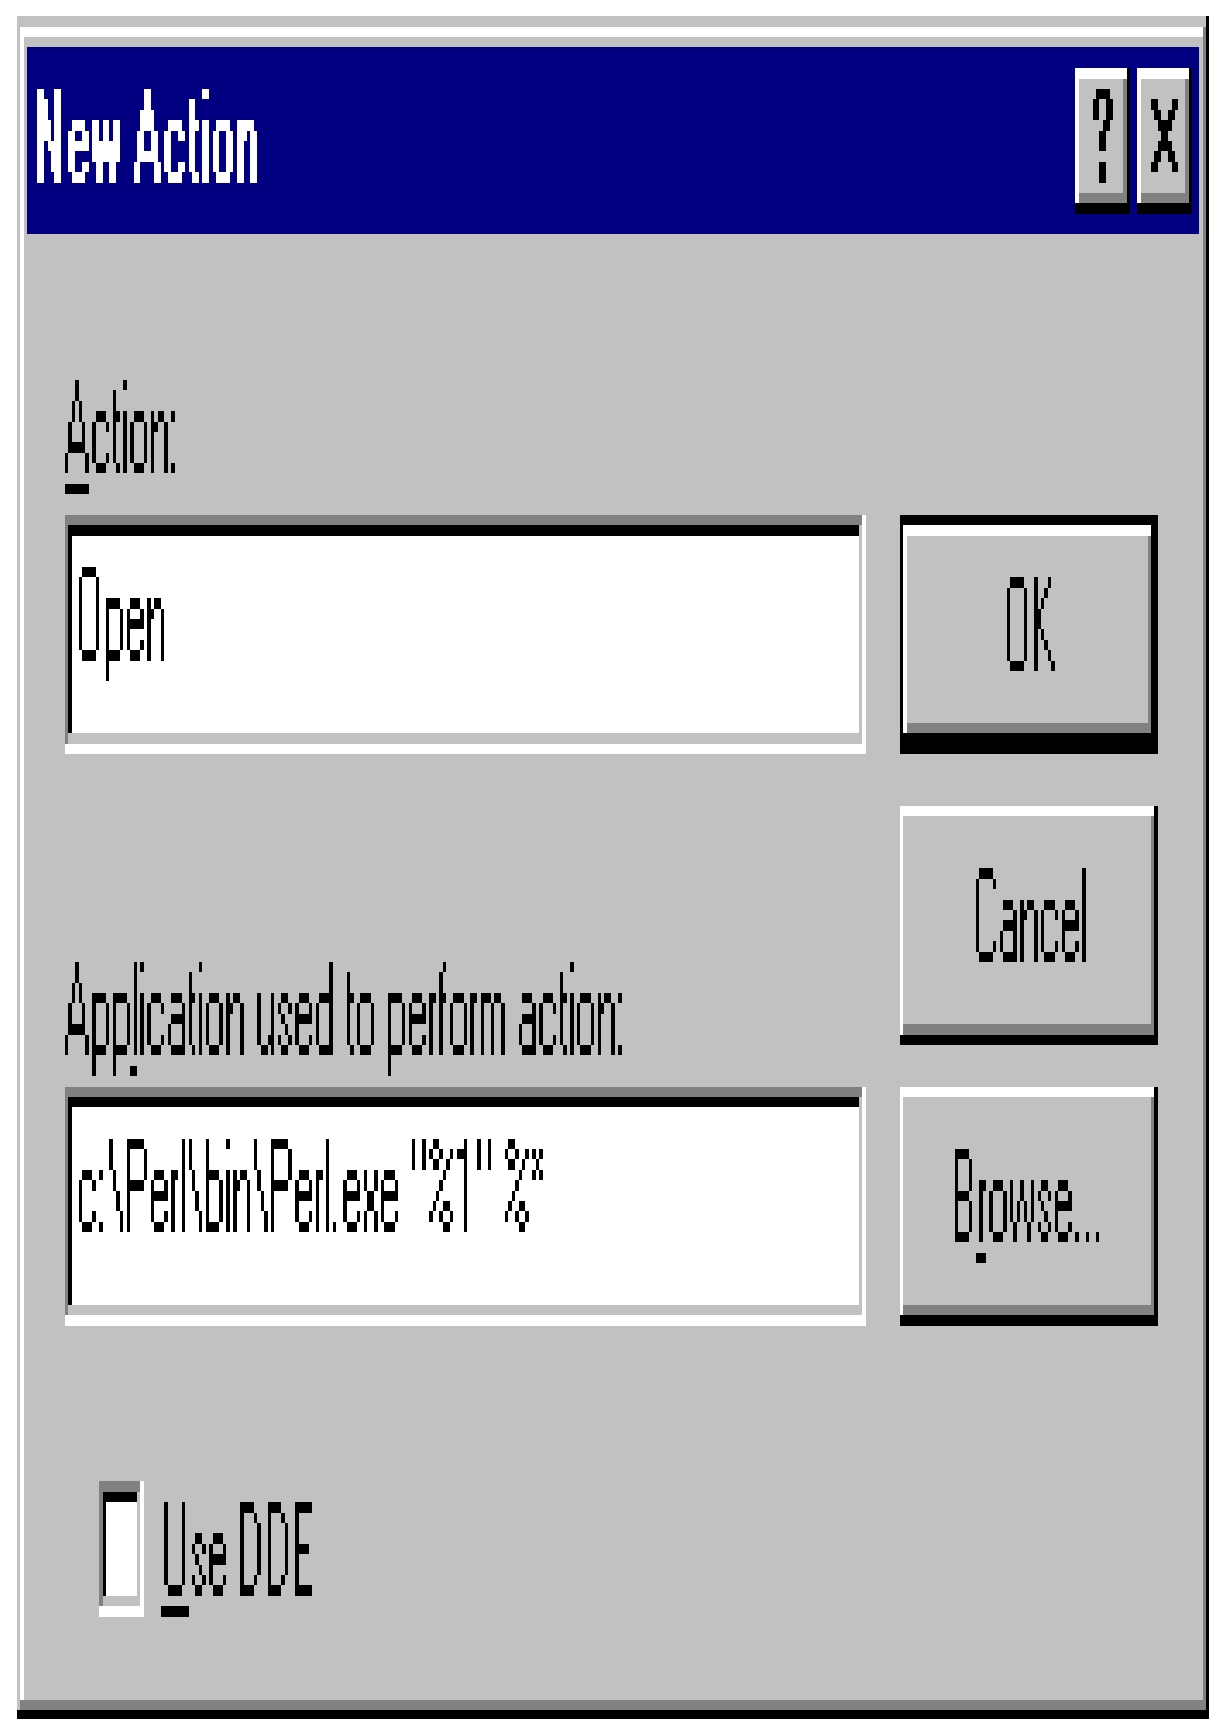
\includegraphics[bb=0mm 0mm 208mm 296mm, width=185.2mm, height=196.3mm, viewport=3mm 4mm 205mm 292mm]{image1.ps}

\noindent 

\noindent This work is licensed under the Creative Commons Attribution-NoDerivs-NonCommercial License. To view a copy of this

\noindent license, visit http://creativecommons.org/licenses/by-nd-nc/1.0 or send a letter to Creative Commons, 559 Nathan Abbott Way, Stanford, California 94305, USA.

\noindent 

\noindent The key terms of this license are:

\noindent 

\noindent Attribution: The licensor permits others to copy, distribute, display, and perform the work. In return, licensees must give the original author credit.

\noindent 

\noindent No  Derivative  Works: The licensor permits others to copy, distribute, display and perform only unaltered copies of the work -- not derivative works based on it.

\noindent 

\noindent Noncommercial: The licensor permits others to copy, distribute, display, and perform the work. In return, licensees may not use the work for commercial purposes -- unless they get the licensor's permission.


\end{document}

% == UNREGISTERED! == GrindEQ Word-to-LaTeX 2008 ==

